\documentclass[a4wide, 11pt]{article}
\usepackage{a4, fullpage, graphicx}
\setlength{\parskip}{0.3cm}
\setlength{\parindent}{0cm}

% This is the preamble section where you can include extra packages etc.

\begin{document}

\title{Human Centred Design Techniques Report}

\author{Lan Yi (ly2715), Pobpawat Pordi(pp2916), Xiaokage Ying(xy1716), Zicong Ma(zm1216)}

\date{\today}         % inserts today's date

\maketitle            % generates the title from the data above

\abstract
need???????????
\\In this report we will discuss the Human Centred Design Techniques that we have used throughout the project. Specifically, we will discuss how we came up with this project idea through initial research and how the use of Human Centred Design techniques affected the project design at during different iterations. 

\section{Initial Research} 


Our initial idea is to create an app that helps people with tracking their expenses, specifically with splitting their bills. We then went on to produce some initial research on the this specific idea. We started off by focusing on young professionals that share expenses with their coworkers and friends. We will discuss in detail the process our initial research below.

\section{Identification of Current State}

In the current market, there do exist many apps that help people with splitting bills and keeping track of their expenses. However, we have also identified that not many people use these apps that are available on the market. Therefore we would like to identify why that is the case. We have done so through some interviews with people of our target audience, and the result can be found in Section \ref{intRes}. As we identified with our interviews, many people dislike the current state of the apps simply because it is not easy enough to use, and it doesn't actually help them with solving their problem of keeping track of the expenses.

\section{Key Design Insights and Proposed Future States}

Based on the problem that we identified through our interviews, we proposed several features:
\begin{itemize}
\item Receipt Scanning - This means that people don't have to go through the pain of entering the items one by one, also saves a lot of their time.
\item Integration with Android Pay/Apple pay to automatically detect their expenses - This kind of automation would mean that users could keep track of their expenses without even opening the app.
\item Learn user's behavior over time - No need to enter repeated bills
\item Allow user to settle debts automatically with other users that uses the app - debts can cancel over time, no need for excess amount of transactions.
\item Paypay/Monzo integration - Allow users to settle debts easily
\end{itemize} 

We believe that with those features, as well as a simple and clean interface, would solve the problem that we identified eariler. We believe that the app that we produce would provide convenience for many young professionals that struggle to track their expenses currently.

\section{Project Iterations}

\subsection{Iteration 1}

We produced an initial mockup to demonstrate some basic functionality of the app, which can be seen in Section \ref{mockup}. The mockup received good feedback from the people we interviewed as they liked the simple interface as well as the receipt scanning functionality: they think that feature can save a lot of their time in the future.

\subsection{Iteration 2}
We introduced our Digital Touchpoint Prototype based on our mockup in Section \ref{dtp}. We also introduced two specific personas, as shown in Section \ref{persona}. We asked them on some Research Questions listed in Section \ref{resQn}, and the feedback has been recorded in Section \ref{feedback}. 
Based on the responses, we decided to keep our app simple, while adding as little features as possible that satisfy the user's need. We would like to keep an clean interface that is easy for the user to navigate around.

\subsection{Iteration 3}
Based on our user feedback from last iteration, we started implementing the application itself.
In this iteration, we introduced Login Page and Home page as well as an add transaction page, some very basic functionality for the app, shown in Section \ref{appIt1}. The user mentioned that they like the simplicity in the design, especially in the Add Transaction page, they mentioned one point for improvement can be adding drop-down menus for the entry fields as well as default options, which can make their life easier while entering the transaction. They also mentioned that they very much look forward to the receipt scanning feature.

\subsection{Iteration 4}
We started implementing the receipt scanning feature as user requested in the previous iteration. However, that feature is not easy to implement, especially when trying to pick out all the items from the receipt one by one, that is especially time consuming. Therefore we decided to implement an easier version of the feature first, and see how the feedback is like on that feature before digging deeper into the more sophisticated aspect of this feature. The progress can be seen in Section \ref{appIt2}. The users liked this feature but they mentioned that they would also like the feature to be able to split out different items in the bill. They think that feature would be especially helpful when going grocery shopping for their friends but different people request different items. They also mentioned that they would like to see the picture that they took before the receipt processed, because they don't want to waste time requesting information from a blurred picture. They also mentioned that they would like easier navigation around the app, since the number of interfaces are getting greater, possibly a menu would be very good.

\subsection{Iteration 5}
We implemented the features that the user suggested in the previous iteration, and the progress can be seen in Section \ref{appIt3}. The users are very impressed with the new features and they also made a couple more suggestions. One user mentioned that they would like to crop the picture after it has been taken, and possibly resize functionality as well. Another mentioned the UI design could be improved, especially with how the menu bar looks and where it is located.

\section{Appendix}

\subsection{Interview Response}
\label{intRes}
Below are the some of the response we had when interviewing young people that just started their professional career.

\begin{itemize}
  \item ‘We end up taking as much time to write down down the items and details of an expense’
  \item ‘Why do I have to enter the same details every time? I'm fed up with it.’
  \item ‘I’m still too lazy to do mental arithmetic.’
  \item 'Why is it so complicated to add a bill?'
  \item 'The app just is not easy to use, too many useless features that I don't need.'
  \item 'Sometimes my friends don't believe me when I tell them that they owe me. It is also very difficult when you tell your coworker that they owe you money.'
\end{itemize}

\subsection{Initial Mockup}
\label{mockup}
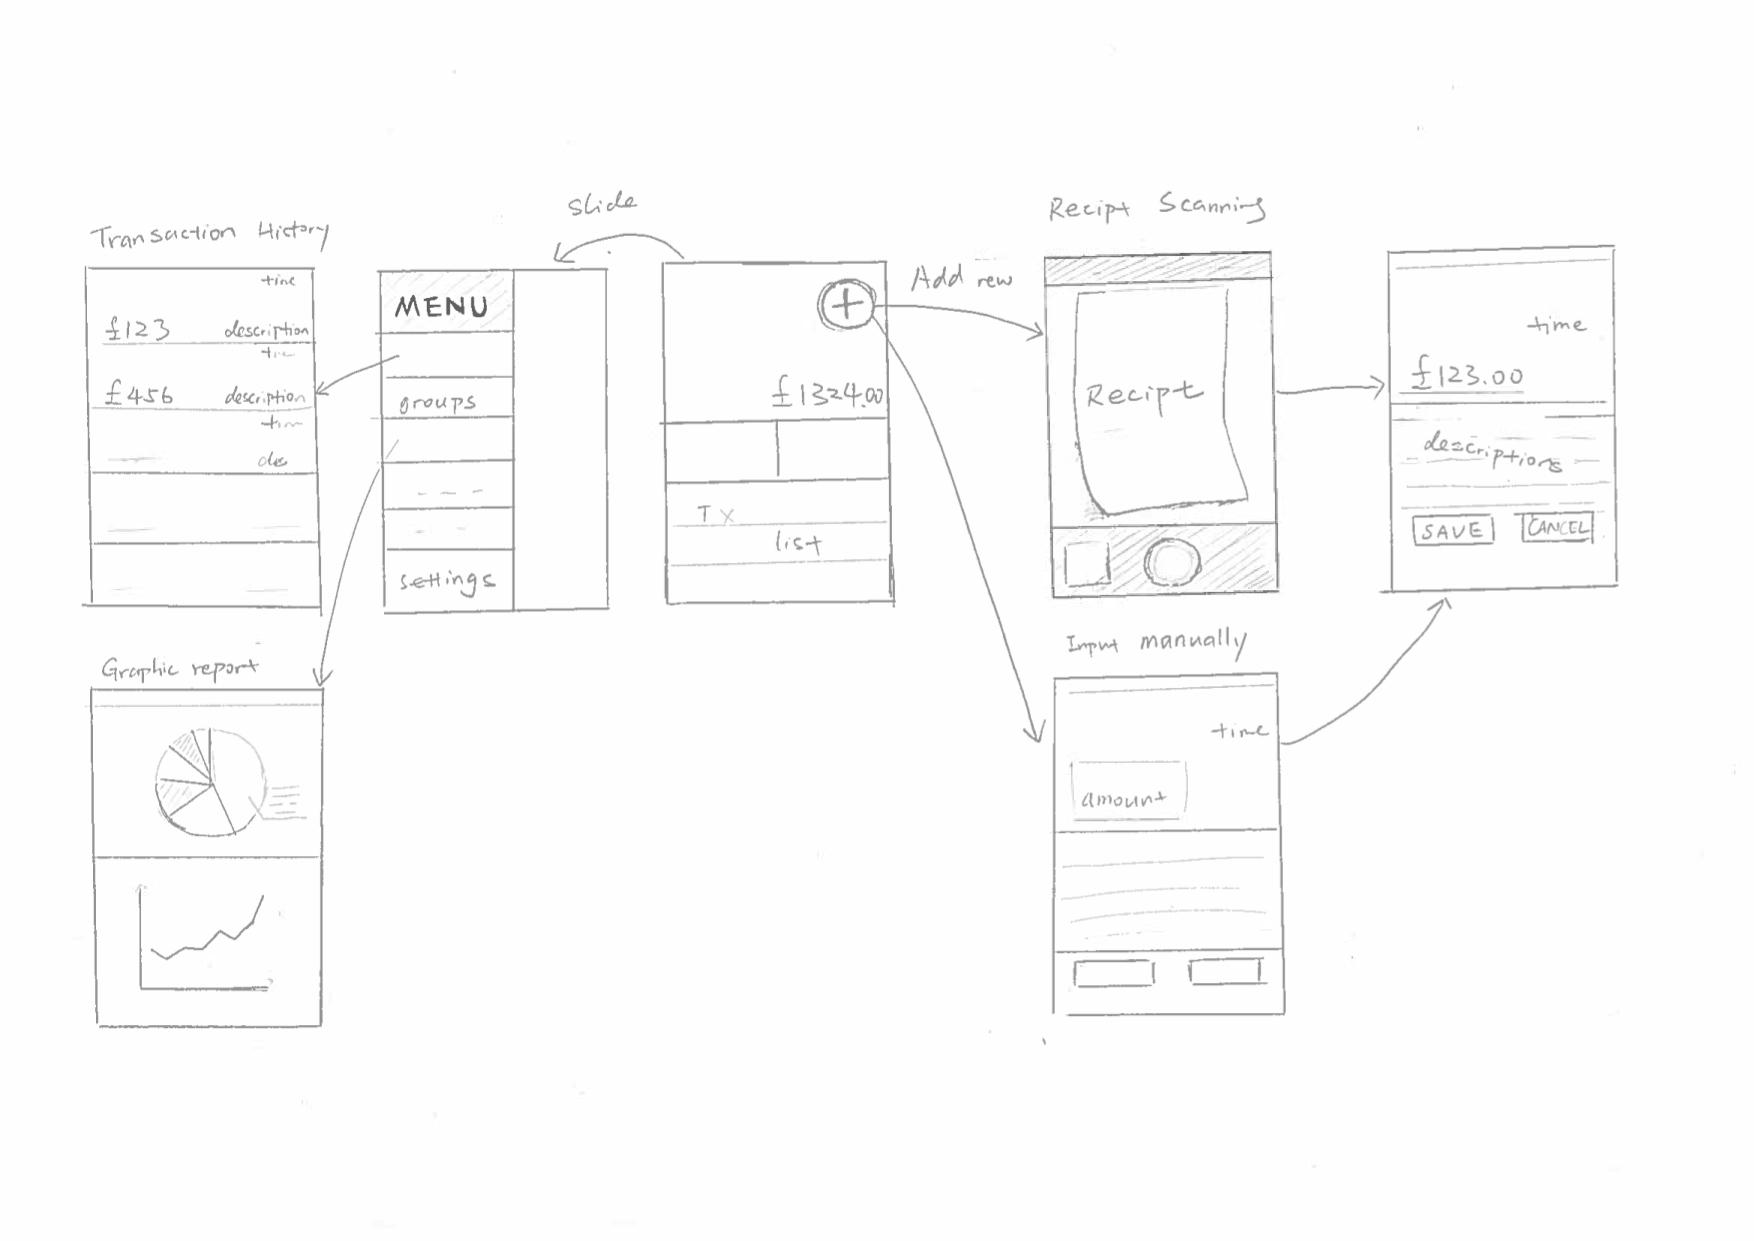
\includegraphics[width=\textwidth]{initialMockup.jpg}

\subsection{Digital Touchpoint Prototype}
\label{dtp}
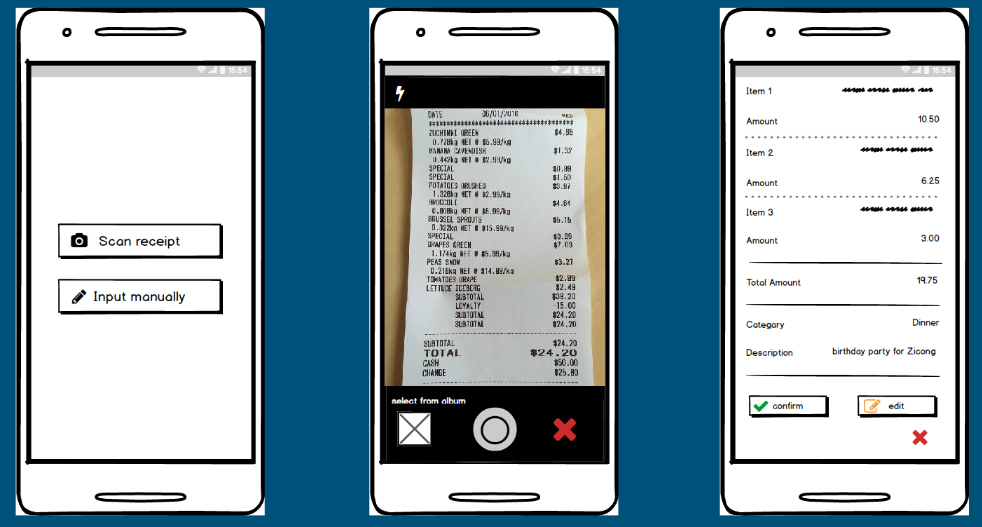
\includegraphics[width=\textwidth]{DTP1.png}
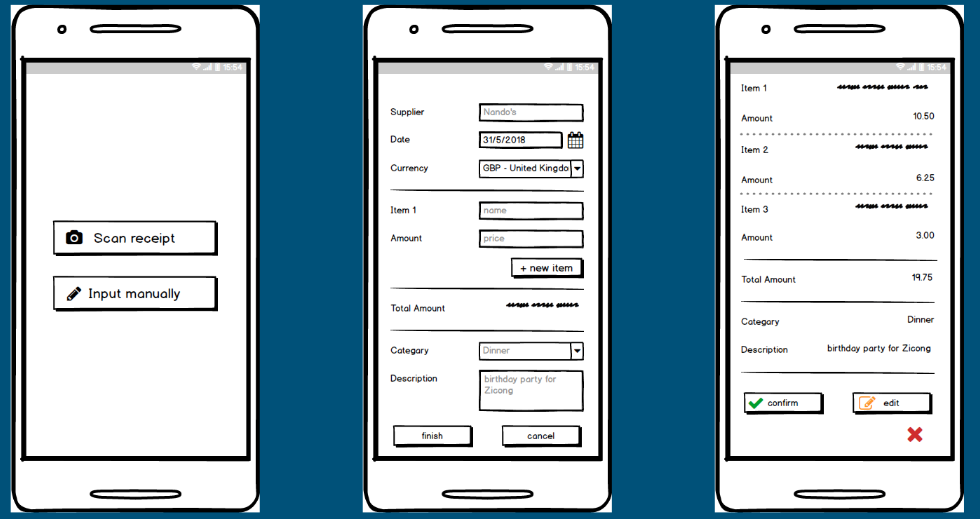
\includegraphics[width=\textwidth]{DTP2.png}

\subsection{Personas}
\label{persona}
\subsubsection{Persona1}
Jane Doe
\begin{itemize}
  \item 22 years old
  \item Did not go to university - went straight into work
  \item Office worker in a Marketing Firm with London average starting salary
  \item Spends most of her time in work 
  \item Hates to spend time on inefficient unnecessary work
  \begin{itemize}
    \item ie. typing out the receipt manually on expense tracker apps
    \item Not a fan of having to do any arithmetic, even with a calculator
    \item Doesn’t like the learning curve on how to use new apps/technology
  \end{itemize}
\end{itemize}
  
Need/Pains: Already likes to track her expenses, however, finds current apps inconvenient, too time consuming and cant convince her friends to use it.

Goals: Be able to easily track expenses without having to spend 5 minutes putting in details every time (preferably with the least amount of hassle)


\subsubsection{Persona2}
John Doe

\begin{itemize}
  \item 23 years old
  \item Recent graduate, currently working at large tech company
  \item Higher-than-average salary
  \item Still leading a student-lifestyle, despite graduating
  \item Nice guy who doesn’t mind paying for the `group
\end{itemize}

Need/Pains:
(Thinking) he’s losing a non-insignificant amount of money from losing track of the expenses and bills he’s paid for his friends

Goals: 
Wants to know exactly which of his friends/coworkers owes him what, and have a record of every time he’s paid for/been paid for.

\subsection{Research Questions}
\label{resQn}
\begin{itemize}
  \item How often do you split the bill with others, per month?
  \item Roughly, could you give us an idea of how much money each bill you split would cost you?
  \item How much money do you think you lose track of, per bill?
  \item How much of monthly expenses are shared? How much is that relative to all your monthly expenses disregarding rent?
  \item If you had to split a bill with a group, how often would you be the one to volunteer to:
  \begin{itemize}
    \item Pay for the group?
    \item Calculate the shares?
    \item Any particular reason why for the above?
  \end{itemize}
  \item Do you use any of the current bill splitting/expense tracking apps?
  \item What do you currently think of that app?
  \begin{itemize}
    \item Does it help you save time/effort?
    \item How many people do you use this app with?
    \item Do the others who you use it with also agree with you?
  \end{itemize}
  \item Have you tried many other apps, or just this one?
  \item What’s your favourite thing about the app? Least favourite?
  \item What’s your first impression on the app?
  \item Do you think it has all the features you’d need?
  \item Do you think the UI is intuitive/simple enough?
  \item What would be your most-used feature?
  \item Do you think your friends/family/coworkers/flatmates would use this too?
\end{itemize}

\subsection{Preliminary Feedback on Research Questions}
\label{feedback}
\begin{itemize}
  \item Focus on keeping it simple
  \item Too many features end up being clutter, even if they’re hidden away in the UI.
  \item Young Professionals are more considerate of their spendings and their shared expenses
Likely due to them being their own money they earn through work and not loans/parents.
  \item Nice guy who doesn’t mind paying for the `group
  \item Most said they liked our mockups, but didn’t care too much about advanced/detailed features.
\end{itemize}

\subsection{Application Iteration 1}
\label{appIt1}
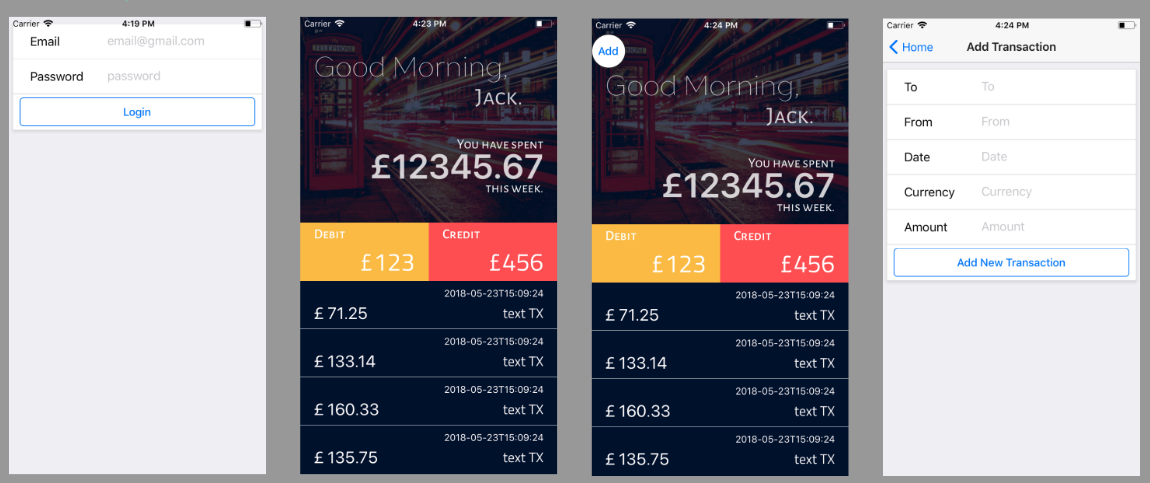
\includegraphics[width=\textwidth]{appIt1.png}

\subsection{Application Iteration 2}
\label{appIt2}
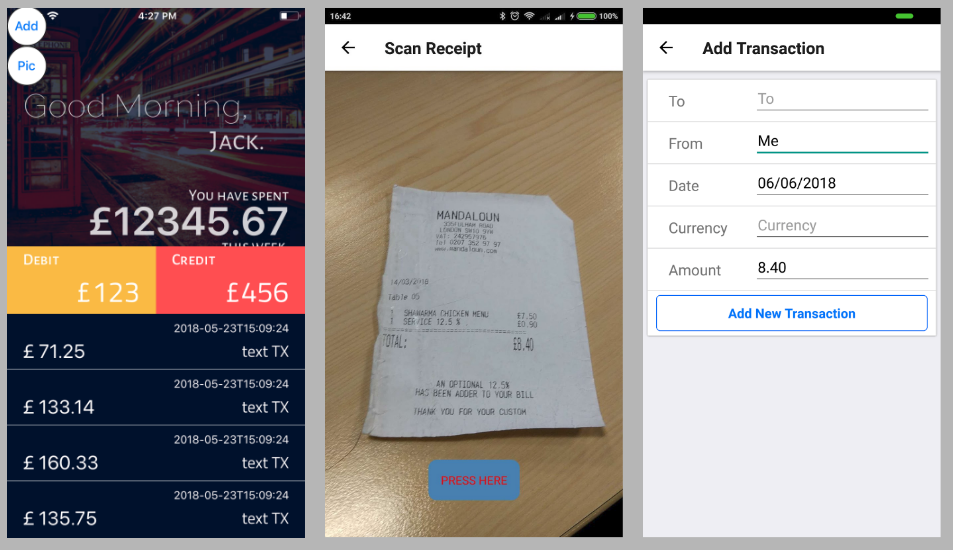
\includegraphics[width=\textwidth]{appIt2.png}

\subsection{Application Iteration 3}
\label{appIt3}
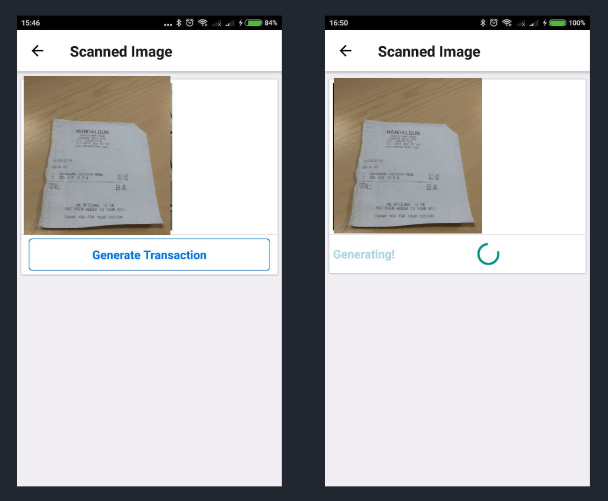
\includegraphics[width=0.75\textwidth]{appIt3.png}

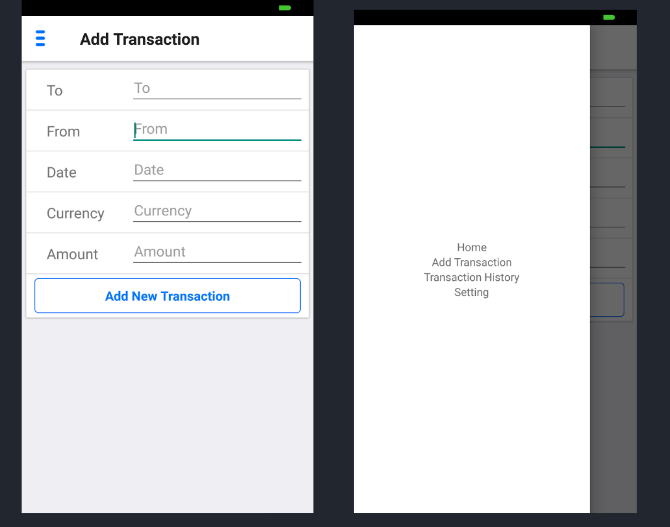
\includegraphics[width=0.75\textwidth]{appIt4.png}

\end{document}